\let\negmedspace\undefined
\let\negthickspace\undefined
\documentclass[journal]{IEEEtran}
\usepackage[a5paper, margin=10mm, onecolumn]{geometry}
\usepackage{lmodern} 
\usepackage{tfrupee} 
\setlength{\headheight}{1cm}
\setlength{\headsep}{0mm}   

\usepackage{gvv-book}
\usepackage{gvv}
\usepackage{cite}
\usepackage{amsmath,amssymb,amsfonts,amsthm}
\usepackage{algorithmic}
\usepackage{graphicx}
\usepackage{textcomp}
\usepackage{xcolor}
\usepackage{txfonts}
\usepackage{listings}
\usepackage{enumitem}
\usepackage{mathtools}
\usepackage{gensymb}
\usepackage{comment}
\usepackage[breaklinks=true]{hyperref}
\usepackage{tkz-euclide} 
\usepackage{listings}                             
\def\inputGnumericTable{}                                 
\usepackage[latin1]{inputenc}                                
\usepackage{color}                                            
\usepackage{array}                                            
\usepackage{longtable}                                       
\usepackage{calc}                                             
\usepackage{multirow}                                         
\usepackage{hhline}                                           
\usepackage{ifthen}                                           
\usepackage{lscape}
\usepackage{xparse}

\bibliographystyle{IEEEtran}

\title{4.3.49}
\author{EE25BTECH11059 - Vaishnavi Ramkrishna Anantheertha}

\begin{document}
\maketitle

\renewcommand{\thefigure}{\theenumi}
\renewcommand{\thetable}{\theenumi}

\numberwithin{equation}{enumi}
\numberwithin{figure}{enumi} 

\textbf{Question}:
Write the equation of the lines for which $\tan\theta = \frac{1}{2}$, where $\theta$ is the inclination of the line, and
\begin{enumerate}
\item[(a)] y intercept $- \frac{3}{2}$
\item[(b)] x intercept $4$
\end{enumerate}
\textbf{Solution 1: }
\begin{table}[H]    
  \centering
  \begin{tabular}{|c|c|}
\hline
\textbf{Variable} & \textbf{Value} \\
\hline
$A$ & $(0,-\frac{3}{2})$ \\
\hline
$m$ & $\frac{1}{2}$ \\
\hline
\end{tabular}
  \caption{Variables Used}
  \label{tab:4.3.49}
\end{table}
\begin{align}
\vec{A}=\myvec{
                0
                \\
                 -\frac{3}{2}  }\\
\text{Let }\vec{M}=\myvec{
                           1
                           \\
                            m
                            }\\
            \vec{M}=\myvec{
                           1
                           \\
                            \frac{1}{2}
                            }
\end{align}
Let eq of line be
\begin{align}
\vec{n^T}(\vec{x}-\vec{A})=0
\end{align}
where,
\begin{align}
\vec{n^T}\vec{M}=0\\
\vec{n}=\myvec{-m
               \\
               1}\\
\vec{n}=\myvec{-\frac{1}{2}
                \\
                1}
\end{align}
Hence eq of line is
\begin{align}
\myvec{-\frac{1}{2}&1}
(\vec{x}-    
\myvec{
           0
           \\
            -\frac{3}{2}
               }   )
=0\\
\myvec{-\frac{1}{2}&1}\vec{x}
=-\frac{3}{2}
\end{align}


Refer to Figure

\begin{figure}[H]
\begin{center}
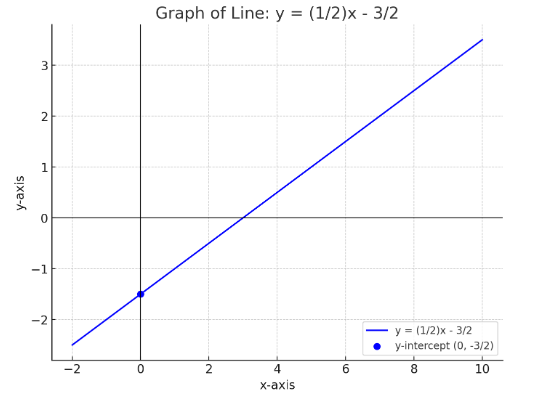
\includegraphics[width=0.6\columnwidth]{figs/grapha.png}
\end{center}
\caption{}
\label{fig:Fig}
\end{figure}
\textbf{Solution 2: }
\begin{table}[H]    
  \centering
  \begin{tabular}{|c|c|}
\hline
\textbf{Variable} & \textbf{Value} \\
\hline
$A$ & $(4,0)$ \\
\hline
$m$ & $\frac{1}{2}$ \\
\hline
\end{tabular}
  \caption{Variables Used}
  \label{tab:4.3.492}
\end{table}
Let $\vec{B}$ be a point on the line 
\begin{align}
\vec{A}=\myvec{
                4
                \\
                 0  }\\
\text{Let }\vec{M}=\myvec{
                           1
                           \\
                            m
                            }\\
            \vec{M}=\myvec{
                           1
                           \\
                            \frac{1}{2}
                            }
\end{align}
Let eq of line be
\begin{align}
\vec{n^T}(\vec{x}-\vec{A})=0
\end{align}
where 
\begin{align}
\vec{n^T}\vec{M}=0\\
\vec{n}=\myvec{-m
               \\ 
               1}\\
\vec{n}=\myvec{-\frac{1}{2}
               \\ 
               1}
\end{align}

\begin{align}
\myvec{-\frac{1}{2}& 1 }
(\vec{x}-    
\myvec{
           4
           \\
            0
               })
= 0\\
\myvec{-\frac{1}{2}&1}\vec{x}
=-2
\end{align}
Refer to Figure

\begin{figure}[H]
\begin{center}
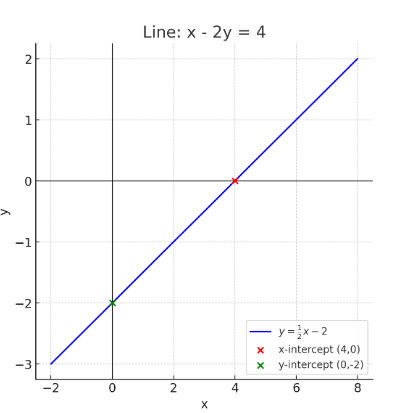
\includegraphics[width=0.6\columnwidth]{figs/graphb.png}
\end{center}
\caption{}
\label{fig:Fig}
\end{figure}
\end{document}  